\documentclass[11pt,a4paper, twocolumn,
swedish, english %% Make sure to put the main language last!
]{article}
\pdfoutput=1

%% Andréas's custom package 
%% (Will work for most purposes, but is mainly focused on physics.)
\usepackage{custom_as}

%% Figures can now be put in a folder: 
\graphicspath{ {figures/} %{some_folder_name/}
}

%% If you want to change the margins for just the captions
\usepackage[size=small]{caption}

%% To add todo-notes in the pdf
\usepackage[%disable  %%this will hide all notes
]{todonotes} 

%% Change the margin in the documents
\usepackage[
%            top    = 3cm,              %% top margin
%            bottom = 3cm,              %% bottom margin
             left   = 1.2cm, right  = 1.2cm %% left and right margins
]{geometry}


%% If you want to change the formatting of the section headers
%\renewcommand{\thesection}{...}



%%%%%%%%%%%%%%%%%%%%%%%%%%%%%%%%%%%%%%%%%%%%%%%%%%%%%%%%%%%%%%%%%%%%%%
\begin{document}%% v v v v v v v v v v v v v v v v v v v v v v v v v v
%%%%%%%%%%%%%%%%%%%%%%%%%%%%%%%%%%%%%%%%%%%%%%%%%%%%%%%%%%%%%%%%%%%%%%


%%%%%%%%%%%%%%%%%%%% vvv Internal title page vvv %%%%%%%%%%%%%%%%%%%%%
\title{SALSA project report}
\author{Andréas Sundström}
\date{\today}


\twocolumn[
\begin{@twocolumnfalse}
\maketitle
\begin{abstract}

\end{abstract}
\end{@twocolumnfalse}
]


%%%%%%%%%%%%%%%%%%%% ^^^ Internal title page ^^^ %%%%%%%%%%%%%%%%%%%%%
%% If you want a list of all todos
%\todolist

\section{Introduction}
The interstellar medium (ISM) contains clouds, among others, atomic
hydrogen HI, which trough quantum mechanical hyperfine structure
electronic transitions emitts electromagnetic radiation with a
frequency of about 1420\,MHz or 21\,cm. This frequency then gets
Doppler shifted depending on the relative radial velocity between us
and the cloud. Therefore by observing the frequency spectrum of the
incoming radiation in the 21\,cm band, it is possible to determine the
the presense and relative radial velocity of clouds in the line of
sight. 


\section{Method}

\clearpage %temporary
\section{Results and Discussion}
\begin{figure}\centering
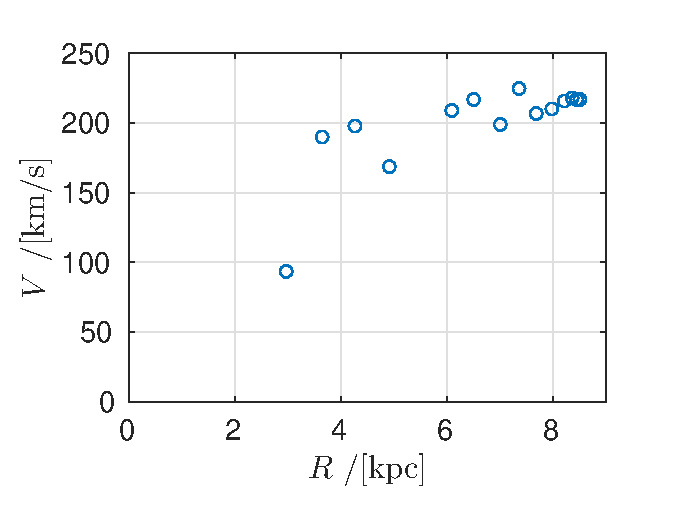
\includegraphics[width=1\linewidth]{rotation_curve.eps}
\caption{Velocity curve for HI clouds in the Milky Way, as observed
  between $20^\circ{-}85^\circ$ Galactic longitude with $5^\circ$
  increments. These velocites are calculated using the circular orbit
  assumption, as well as assuming that the cloud with the highest
  radial velocity is moving tangent to the line of sight. }
\label{fig:rot}
\end{figure}

\begin{figure}\centering
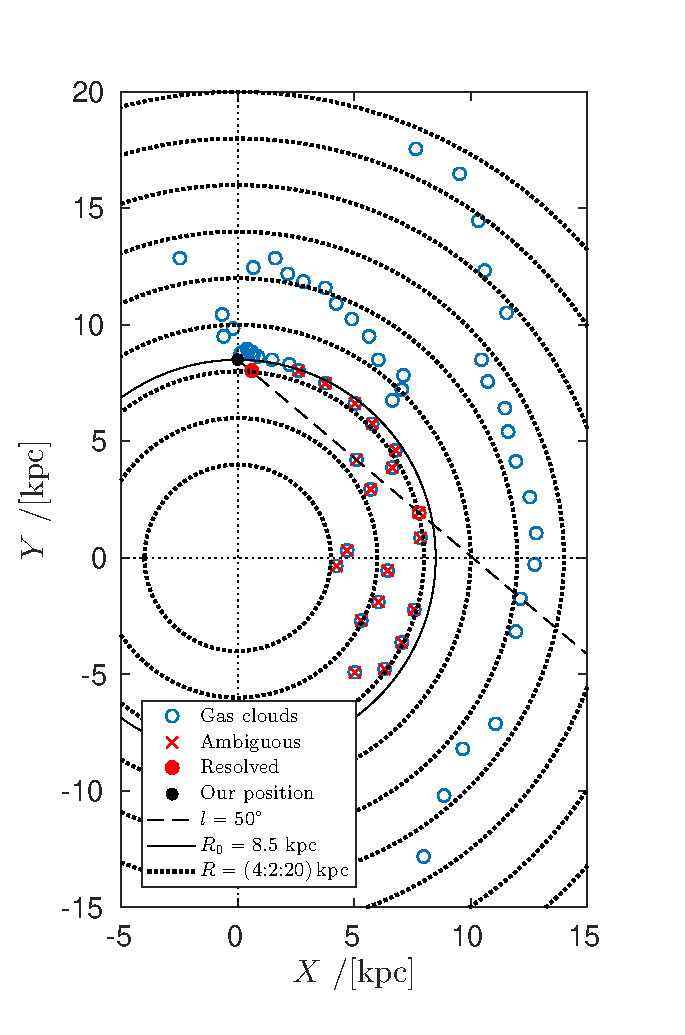
\includegraphics[width=1\linewidth]{gas_clouds.eps}
\caption{Position of HI clouds in the Milky Way. The positions are
  calculated using the assumptions that all clouds have circular
  orbits and that their orbital velocities are
  $V_0=\unit[220]{km/s}$. For some of the coulds there are two
  possible solutions to their position (red crosses). This ambiguity
  problem have been resolved for one cloud on $l=50^\circ$ (red ring,
  correct position filled in). }
\label{fig:clouds}
\end{figure}

\begin{figure}\centering
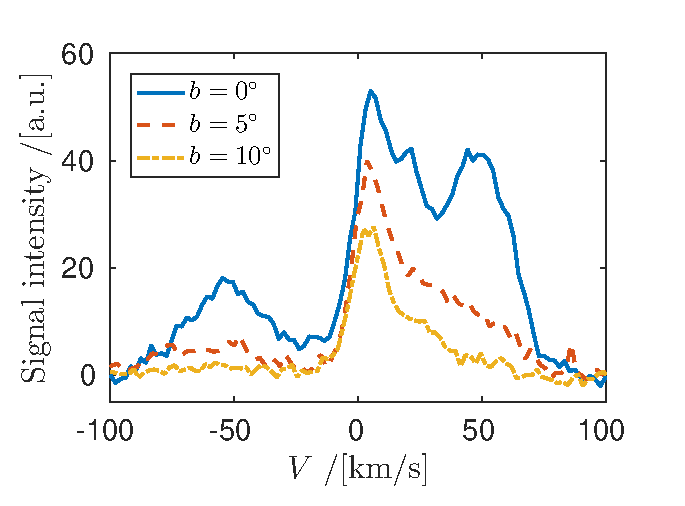
\includegraphics[width=1\linewidth]{ambiguity.eps}
\caption{Velocity spectra to resolve the ambiguity problem for
  $l=50^\circ$. By observing that that the peak near $V=0$ remains for
  different Galactic latitudes, $b$, we can conclude that this gas
  cloud has to be much closer to us than the two others which can be
  seen at $b=0^\circ$. }
\label{fig:ambiguity}
\end{figure}



\section{Conclusions}











%%%%%%%%%%%%%%%%%%%%%%%%%% The bibliography %%%%%%%%%%%%%%%%%%%%%%%%%%
%\newpage
%% This bibliography uses BibTeX
%\bibliographystyle{ieeetr}
%\bibliography{references}%requires a file named 'references.bib'
%% Citations are as usual: \cite{example_article}

%%%%%%%%%%%%%%%%%%%%%%%%%%%%% Appendices %%%%%%%%%%%%%%%%%%%%%%%%%%%%%

%%%%%%%%%%%%%%%%%%%%%%%%%%%%%%%%%%%%%%%%%%%%%%%%%%%%%%%%%%%%%%%%%%%%%%
\end{document}%% ^ ^ ^ ^ ^ ^ ^ ^ ^ ^ ^ ^ ^ ^ ^ ^ ^ ^ ^ ^ ^ ^ ^ ^ ^ ^ ^
%%%%%%%%%%%%%%%%%%%%%%%%%%%%%%%%%%%%%%%%%%%%%%%%%%%%%%%%%%%%%%%%%%%%%%

